\documentclass[a4paper, 12pt]{article}
\usepackage{fontspec} 
\usepackage[utf8]{inputenc}
\usepackage[russian,english]{babel}
\setmainfont{Times New Roman}
\renewcommand{\baselinestretch}{1.5} 


 % для компиляции теперь нужно использовать XeLaTex 
\usepackage{amsfonts}
\usepackage[paper=a4paper,top=13.5mm, bottom=13.5mm,left=20mm,right=20mm,includefoot]{geometry}
\usepackage{indentfirst}
\usepackage{dsfont}
\usepackage{graphicx} 
\graphicspath{{images/}} 
\setlength\fboxsep{3pt} 
\setlength\fboxrule{1pt} 
\usepackage{wrapfig} 
\usepackage{amsmath}
\usepackage{amsthm}
\renewcommand{\proofname}{Доказательство}

\DeclareMathOperator*{\argmin}{arg\,min}
\newcommand{\inde}{\perp\!\!\!\perp}


\theoremstyle{definition}
\newtheorem{definition}{Определение}[section]


\theoremstyle{plain}
\newtheorem{lemma}{Лемма}[section]
\newtheorem{svoistvo}{Свойство}[section]
\newtheorem{theorem}{Теорема}[section]


\title{Исследовательский проект по инстуциональной экономике}
\date{\today}

\begin{document}
\maketitle

\noindent{\bf Аннотация }-- ...

\section{Введение}
Мы устверждаем, что в существуют рынки на которых присутствует сразу несколько игроков со стороны спроса на труд в одном регионе. 
\section{Обзор литературы}

Большинство теорий, связанных с рынком труда, предполагает наличие положительной зависимости уровня заработных плат и продолжительности времени работы в конкретном месте. Наиболее известными работами, демонстрирующими данный эффект, являются статьи Walter Oi (1962) и Jacob Mincer (1974). Однако существуют такие рынки труда, где некоторые исследователи выявляют отрицательную зависимость. Именно таковым и является академический рынок труда, привлёкший наше внимание. 
	Сперва обратимся к моделе, описанной в статье Michael R. Ransom (1993). Автор привёл эмпирическое доказательство того, что с увеличением времени работы профессоров в одном университете их заработная плата падает. Он продемонстрировал выводы трёх различных исследований, получивших несильно разнящиеся результаты, подтверждающие его основную гипотезу. Первое из них - Carnegie Commission National Survey of Higher Education: Faculty Study (1969) заключило что, индивиды, проработавшие как минимум 30 лет в одном университете, зарабатывают примерно на 15%  меньше тех, кто проработал менее двух лет. При этом эффект ярче выражен для более престижных университетов. Важно отметить, что регрессия строилась с поправкой на учёную степень, научную область, пол, расу, качество института, диплом которого получен, продолжительность контракта и контролируемость нанимающего учреждения частным сектором. 
	Результаты исследования American Council on Education's (1973) были следующими:  для исследовательских университетов заработная плата снижается примерно на 0.4% с ежегодным ростом сеньорити (условимся так называть продолжительность времени работы в конкретном месте). 
	Другое исследование, упомянутое автором, - Survey of the American Professoriate (1977). Для всей выборки университетов корреляция между заработными платами и сеньорити не являлась существенной, однако, для исследовательских университетов заработные платы действительно снижались в ростом сеньорити. Эффект наиболее выражен для профессоров с 16-20 годами сеньорити, которые зарабатывают примерно на 7% меньше нежели те, у кого сеньорити не более двух лет (с поправкой на опыт, образование и другие факторы). 
	По результатам всех трёх исследований заключается, что смена места работы может увеличить заработную плату профессора примерно на 5-6%. Также величина снижения заработных плат зависит от академической сферы: для большинства областей падение составляет 0.5%, в то время как бухгалтерский учёт и экономика демонстрируют более 1% ежегодно. 
	Далее Michael R. Ransom оценивает собственную модель на данных университета Аризоны и приходит к выводу: заработные платы падают примерно на 1% c ежегодным ростом сеньорити - эффект более значимый в сравнении с упомянутыми ранее исследованиями. 
	После всех описанных выше эмпирических результатов Michael R. Ransom заключает, что действительно можно говорить о существовании отрицательной связи заработной платы и сеньорити. Автор приводит различные объяснения замеченного феномена. Одно из которых - более способные профессора имеют множество альтернатив, в то время как менее способные вынуждены оставаться на прежнем рабочем месте. Эта идея и лежит в основе моделей Milton Harris and Bengt Holmstrom (1982) и Lazear (1986). Поскольку первоначально фирма не знает о способностях работника, она предлагает стартовую заработную плату. В результате некоторые работники остаются недооценёнными. Другие фирмы идентифицируют таких работников и стараются их нанять, предлагая более высокую заработную плату. Получается, что более «высококачественные» работники получают более высокую заработную плату, а работники с высоким сеньорити имеют тенденцию быть «низкокачественными» и получать более низкую заработную плату. Тем не менее остаётся неясным, каким образом измерять «качество» работников. В качестве одного из способов оценки продуктивности авторы предложили число публикаций. Оказалось, что профессора с высоким сеньорити несильно отличаются количеством публикаций о тех, кто работает недолго в данном университете. Авторы пришли к выводу, что продуктивность или же «качество» работников не может служить адекватным объяснением отрицательной зависимости заработных плат и продуктивности.
	Продолжая поиски ответа на поставленный вопрос, Michael R. Ransom строит модель монопсонистической дискриминации. Он предполагает наличие одного университета в городе, поэтому для смены работы профессору необходимо переехать, что влечёт за собой определённые издержки. Если издержки высоки, агент предпочтёт остаться в прежнем городе (продолжительность работы в одном университете будет расти), а заработная плата будет ниже возможной предложенной университетом в каком-либо другом городе. Однако данная модель не предсказывает, что зарплаты будут падать с ростом сеньорити. Оценённый коэффициент регрессии смещён, поскольку мы не можем включить в неё ненаблюдаемую компоненту издержек переезда. 
	Теперь, когда мы пронаблюдали на монопсоническом рынке эффект падения заработных плат с увеличением сеньорити на примере различных эмпирических исследований и рассмотрели математическую модель, встаёт вопрос: будет ли иметь место рассматриваемый феномен на рынке олигопсонии? Сперва обратимся к исследованию, которое в принципе отрицает существование выявленного феномена, затем уделим внимание особенностям олигопсонического рынка.
	Позднее вышла статья авторов William J. Moore, Robert J. Newman, Geoffrey K. Turnbull (1998), получивших совершенно иные результаты. Отрицательная зависимость  между заработной платой и сеньорити полностью исчезла, когда в модель включили более исчерпывающие оценки продуктивности индивидов, такие как количество публикаций, цитируемость и многие другие. В качестве выборки авторы использовали профессоров, нанятых на программы Ph.D по экономике в 9 государственных университетов. Для усовершенствования предыдущих моделей продуктивность профессоров стали измерять в трёх сферах: исследования, преподавание и управление. Каждой из них был присвоен свой вес в зависимости от целевой функции кафедры. При этом вводилось предположение, что  исследования являлись самой важной компонентой. Для получения градации качества статей, авторы разделили публикации на два типа по отношению к журналу, в котором были напечатаны. Также была введена переменная, отвечающая за цитируемость: как часто другие исследователи ссылались на данную статью. Качество преподавания оценивалось с помощью дамми переменной, которой присваивалась единица в случае, если профессор когда-либо получал награду за преподавание. И последняя оценка продуктивности - количество лет на должности заведующего кафедрой в высшем учебном заведении как показатель управленческих навыков. Также в модель были включены дополнительные дамми переменные, такие как пол индивида, язык страны (английский-1/не английский-0) и рейтинг университета, где получал Ph.D (топовый-1/ не топовый-0). 
	В результате, базовая регрессия оценённая на опыт и синьорити даже с добавлением количества публикаций выявляет отрицательную зависимость заработных плат и продолжительности времени работы в конкретном университете. Однако по мере расширения модели и добавления в неё других вышеописанных переменных наблюдаемая ранее связь исчезает. Профессора с большим сеньорити получают заработную плату относительно меньшую лишь потому, что многие из них менее продуктивны в сравнении в теми, у кого сеньорити ниже.
	Теперь обратимся к статье V. Bhaskar, Alan Manning and Ted To (2002), которая поможет нам понять природу олигопсонии. Авторы говорят,  что монопсония - крайне нереалистичное предположение о функционировании рынка труда; олигопсония же представляет собой более подходящую структуру. Она описывает ситуацию, когда работодатели обладают рыночной силой, несмотря на то, что конкурируют друг с другом. 

\section{Модель}

Многие статьи рассматривают академический рынок труда  как монопсонию (ссылки на статьи). Мы утверждаем, что существуют также рынки олигопсонического типа и совсем не очевидно, что на них будет наблюдаться тенденция к понижению зароботной платы.  Мы рассмотрим модель олигпсонического рынка труда в рамках которой у профессора будет выбор либо остаться в своем регионе и пойти в один из университетов, либо уехать, но понести издержки переезда. Модель будет строится на основе модели монопсонического рынка из статьи Seniority and Monopsony in the Academic Labor Market
Michael R. Ransom (1993). Из неё мы возьмём ...  

Пусть существует рынок в рамках одного города, где присутствует $n$ университетов, предъявляющие спрос на одних и тех же академических работников. Обычно в США в одном городе находится лишь несколько ВУЗов, которые могли бы предъявлять спрос и на одну и ту же рабочую силу, но для общности мы пока буем предполагать, что их $n$. Рынок академических работников основан в своем большинстве на личном взаимодействии, так как преподаватели являются единственными экземплярами предлагающие именно такую комбинацию способностей. Это сильно отличает академический рынок труда от многих других (неплохо бы ссылку). В следствии этого, каждый университет выбирает какую зарплату предложить отдельно для каждого работника. Зарплату предложенную $i$ университетом мы будет обозначать $w_i$. Также будет существовать рыночная заралата $w_m$, именно с такой зарплатой университету придется нанять работника, если профессор, которому предложили зарплату $w_i$ откажется. Университет минимизирует свои ожидаемые издержки: 
\[
EC(w_i) = p_i(w_m, w_i, m, w_{j \neq i})w_i + (1 - p_i(w_m, w_i, m, w_{j \neq i}))w_m
\]

Как мы видим, в зависимости от предложенной зарплаты, зарплаты предложенной другими университетами, зарплаты по рынку и издержкам переезда будет устанавливаться некоторое распределение, случайным исходом для которой будет являться выбор, который сделает преподаватель. Как и в модели с монопсонией мы будем предлагать для простоты, что агенты обладают полной информацией, и единственный источник случайности заключается в выборе профессора одного из университетов. Мы можем предложить, что функция $p_i ( w_m, w_i, m, w_{j \neq i}) $ имеет следующий вид: 
\[
p_i( w_m, w_i, m, w_{j \neq i}) = \frac{p_i(w_i - w_m + \delta m) w_i}{\#\{w_j : w_i = w_j\}}\mathds{1} \{ w_i \geq w_ {i \neq j}\}
\]
Профессор сравнивает предложенную ему зарплату некоторым университетом с зарплатой рынка и своими дисконтированными издержками. Более того, в виду наличия функции индикатора максимальной цены, преподаватель будет рассматривать лишь тот университет, который предложил ему наибольшую зарплату. Всем остальным вузов придется нанимать преподавателя на общем рынке. В виду присутствия ненаблюдаемых факторов решение всё равно остается случайным. 

Возможен также случай, когда несколько университетов предложат максимальную зарплату. Именно этот фактор учитывает знаменатель дроби, который означает, что вероятность попасть в конкретный ВУЗ делится на количество ВУЗов предложивших такую же зарплату. 

Проанализируем поведение стороны спроса на рынке. В статье Olygopsony and Monopsonistic Competition in Labor Markets Bhaskar, A. Manning, Ted To (2002)  рассматриваются различные варианты взаимодействия игроков на олигпсоническом рынке.  Мы будем предполагать, что они не вступают в сговор. Мы считаем, что такая предпосылка вполне оправдана, так как профессора являются единичным товаром, в следствии чего доход от его приобретения почти невозможно разделить легальным путем. 

Заметим, что если вуз устанавливает зарплату ниже чем его конкуренты, то он сталкивается с рыночной ценой с вероятностью 1, соответсвенно в симметричном равновесии  вузы должны установить одинаковую зарплату. И должно быть выполнено следующее условие для каждого конкретного учебного заведения
\[
p_i(w_i - w_m + \delta m) w_i + (1 - p_i(w_i - w_m + \delta m))w_m = \frac{p_i(w_i - w_m + \delta m) w_i}{n} + (1 -\frac{ p_i(w_i - w_m + \delta m)}{n})w_m \leq w_m
\]
Это уравнение означает, что конкретному ВУЗу не выгодно повысить зарплату на любую положительную величину, чтобы повысить вероятность прихода к нему профессора, и более того, в равновесии ожидаемые издержки отдельного ВУЗа не должны превышать рыночную цену на учёного, иначе он обязательно переключится на эту альтернативу
Раскрывая скобки мы получаем 
\[
\frac{(n-1)p_i(w_i - w_m + \delta m) w_i}{n} = \frac{(n-1) p_i(w_i - w_m + \delta m) w_m}{n}
\]
\[
w_i = w_m
\]

Мы видим, что в случае такой конкуренции будет установлено равновесие в котором каждый вуз предлагает одинаковую зарплату равную рыночной, ученый в свою очередь с вероятностью $p(\delta m)/n$ выбирает один из вузов, и с вероятностью $1 - p(\delta m)$ уезжает из города. Соответсвенно мы не ожидаем увидеть на данных тенденцию к понижению зарплаты на таких рынках. Более того, можно сказать, что почти не существует ситуаций, когда несколько ВУЗов в одном городе предлагают профессору рыночную зарплату. Но так как теперь ВУЗам безразлично с точки зрения модели, какого профессора брать, то со стороны спроса вполне может остаться только один агент. Также естественно предположить, что не за каждого профессора идёт такая борьба на рынке труда, следовательно на данных мы ожидаем увидеть не противоположный эффект, как в предыдущих статьях, но более слабый. 

Мы выяснили, что в случае такой ситуации на рынке мы не ожидаем понижения зарплат. Аналогично монопсонической модели мы можем предложить, что в течение жизни профессора через равные промежутки времени перед ним встаёт снова выбор, уехать или нет.  Его зарплата в этот момент обновляется в результате реализации случайного события.  Именно на основании такого анализа авторы статьи [1] и пришли к выводу о падении зарплат. В связи с этим мы можем предположить, что конкуренция за профессора не ведется на протяжении всех периодов, что по нашему мнению является вполне осознанной предпосылкой, так как профессора редко меняют университет, исходя из этого можно заключить, что и в конкуренцию за профессоров ВУЗы вступают редко. Следовательно в какие то периоды, мы будем снова оказываться в случае монопсонии. Тогда на протяжении всех периодов зарплата будет вести себя скачкообразно, если профессор всё это время оставался в городе. % если будет не хватать места, то я опишу математически этот эффект

В динамике мы получили, что эффект понижения зарплат на таких рынках будет наблюдаться, только теперь он будет  слабее, чем на рынках, где лишь один университет определенного уровня.

\section{Кейс}

В качестве примера, иллюстрирующего вышеописанную модель, будет рассмотрен Хьюстонская система университетов. Во-первых, университеты внутри этой системы независимы и примерно одного ранга (Tier 2), то есть между ними существует конкуренция за рабочую силу. Во-вторых, в Хьюстоне также присутствует достаточно большое количество университетов второго ранга, например, Техас Саутерн и Университет Конкордия. Все эти учебные заведения расположены в пределах города Хьюстон и его пригорода. Исходя из данной информации можно сделать вывод, что рынок академического труда города Хьюстон можно рассматривать как олигопсонию. Заметим, что это справедливо только для университетов второго ранга и ниже, потому что в данном городе присутствует только один университет первого ранга Райс.

Данные о работниках Хьюстонской системы находятся в открытом доступе на сайте: http://salaries.texastribune.org/university-of-houston/. Перед началом анализа данные были обработаны. Сначала была проведена очистка данных от работников департаментов, занимающихся административной и обслуживающей деятельностями. Далее были оставлены только работники, занимающиеся преподаванием, то есть профессоры. Наконец, была добавлена переменная $seniority$, показывающая сколько полных лет индивид проработал в данном университете.
Для анализа будут использованы следующие переменные из ранее упомянутой базы данных: $rate$ --- уровень заработной платы, $sex$ --- пол индивида (1 --- мужчина), $Fullp$ --- является ли индивид "полным профессором", $Type$ --- полный рабочий день или частичный, $Foreign$ --- показывает расу (0 --- европеоидная, 1 --- остальные).

Дескриптивная статистика выборки:

\begin{center}
\begin{tabular}{|c|c|c|}
\hline 
• & lograte & seniority \\ 
\hline 
Среднее & 11.47 & 13.35 \\ 
\hline 
Медиана & 11.45 & 10.00 \\ 
\hline 
Стандартное отклонение & 0.39 & 12.11 \\ 
\hline 
N=1016 & • & • \\ 
\hline 
\end{tabular} 
\end{center}

\begin{center}
\begin{tabular}{|c|c|c|}
\hline 
• & N & \% \\ 
\hline 
Мужчины & 688 & 67.72 \\ 
\hline 
"Полные" профессора & 351 & 34.55 \\ 
\hline 
Работающие полный день & 994 & 97.83 \\ 
\hline 
"Европейцы" & 634 & 62.40 \\ 
\hline 
\end{tabular} 
\end{center}

Воспользуемся Минцеровским уравнением для того, чтобы оценить влияние рабочего стажа на заработную плату:

$$lograte=\alpha_1+\alpha_2 Sex+\alpha_3 Seniority +\alpha_4 Fullp+\alpha_5 Type +\alpha_6 Foreign$$

где $lograte$ --- логарифм заработной платы.

Значения полученных коэфициентов:

\begin{center}
\begin{tabular}{|c|c|c|}
\hline 
• & Оценка коэфициента & Стандартное отклонение оценки \\ 
\hline 
Свобдный член & 10.79754 & 0.07216 \\ 
\hline 
sex & 0.12098 & 0.02134 \\ 
\hline 
seniority & -0.00588 & 0.00095 \\ 
\hline 
fullp & 0.51297 & 0.02447 \\ 
\hline 
type & 0.48461 & 0.06923 \\ 
\hline 
foreign & 0.07161 & 0.02056 \\ 
\hline 
\end{tabular} 
\end{center}

Все полученные коэфициенты значимы даже при очень маленьких уровнях значимости ($\alpha<0.001$).

В нашем примере $R^2=0.36$. Такое значение позволяет нам думать, что зависимость однозначно существует, но частично остаток должен объясниться с помощью дополнительных регрессоров, например, опыт или возраст и квадрат этих величин. В данном уравнении не было использовано таких переменных, ибо в нашей базе данных не было возраста преподавателей, а восстанавливать его достаточно сложно.
Также коэффициент, который мы получили при seniority больше, чем аналогичный у Ransom 1993. Этот факт можно объяснить как раз из-за потерянных нами важных переменных (в уравнении Минцера возраст является одним из важнейших показателей).

Также, возможные проблемы могут возникать из-за того, что выборка не является репрезентативной. Такой вывод можно сделать исходя из графика плотности логарифма заработной платы: в идеальной ситуации логарифм заработной платы должен быть распределен нормально, однако, в здесь наблюдается смещение в сторону более высоких зарплат профессоров.


\begin{center}
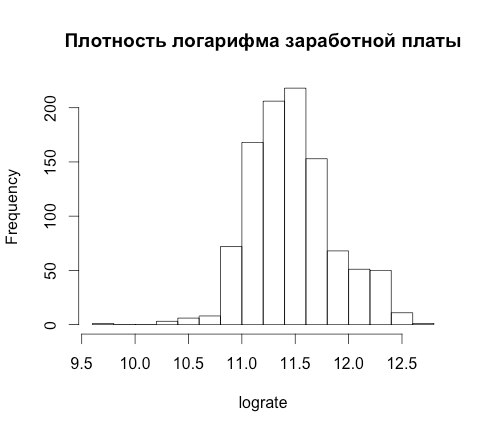
\includegraphics[scale=0.5]{image1}
\end{center}

\section{Заключение}




\end{document}



